\subsection{FRIIS Equation and Shannon-Hartley Capacity}
\subsubsection{FRIIS Equation}
We use FRIIS equation to calculate the \textbf{reception's power}, we used the following parameters:

\begin{align*}
	G_{Tx}= 3 dBi\\
	G_{Rx}= 3 dBi\\
	c = 3 \times 10^8 \ \left[\frac{m}{s}\right] \\
	fc = 433 MHz\\
	P_{Tx} = 40 dBm\\
	Sensivity = -106 dBm
\end{align*}

And FRIIS equation:

\begin{equation}
	P_{Rx} = P_{Tx} + G_{Tx} + 20l\log_{10}\left(\frac{c}{fc}\right) -20\log(4\pi r)
\end{equation}

We got the following results:

\begin{figure}[!htbp]
	\centering
	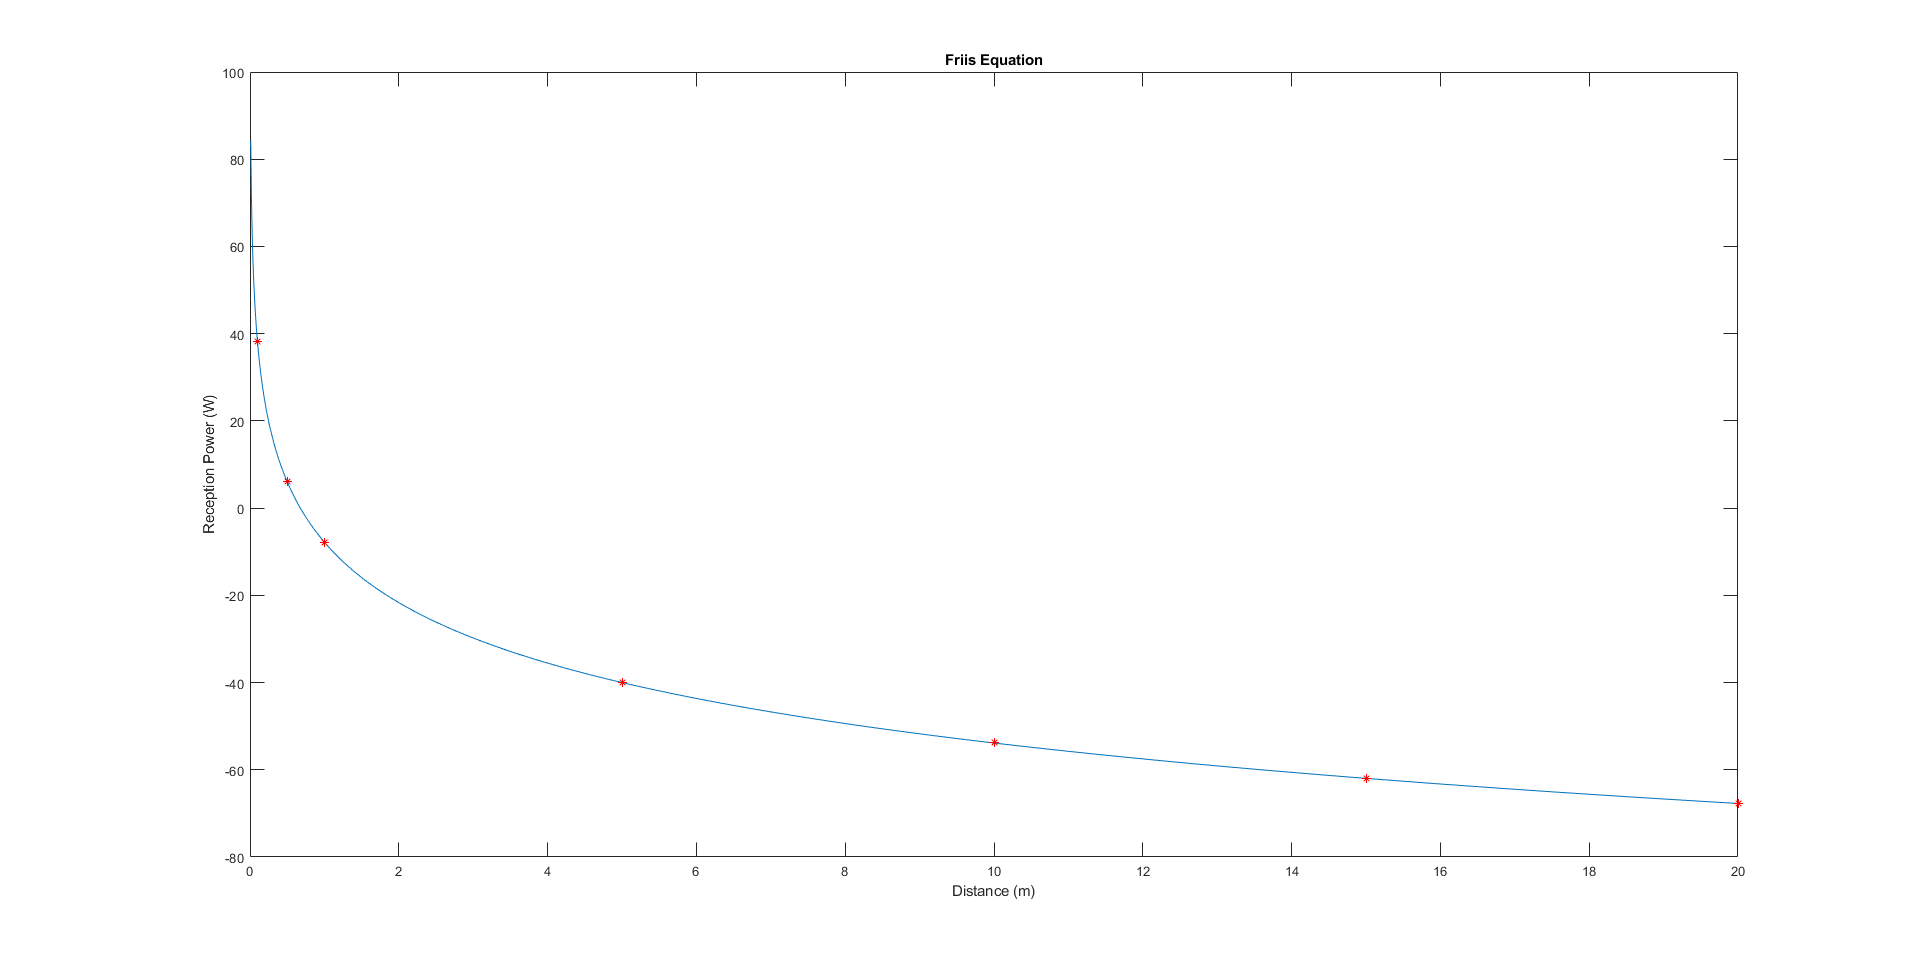
\includegraphics[width=9.5cm]{images/friis.png}
	\caption{Result of $P_{Tx}$}
\end{figure}

As we can see, our receptor could receive transmissions along the testing distance because of the fact the sensivity was $-106 dBm$. However during the transmission, it was show how the channel disturbed our information while it was travelling.

\subsubsection{Shannon-Hartley Capacity}
We use Shannon-Hartley equation to calculate Channel's Capacity. We consider a bandwidth of $25 kHz$ because this is the global use of bandwidth, this might change in some countries. \cite{teleradio_2020}

Shannon-Hartley Capacity Equation:
\begin{equation}
	C = B\log_{2}\left(1+\frac{S}{N}\right)\\
\end{equation}

We got the following results:

\begin{figure}[!htbp]
	\centering
	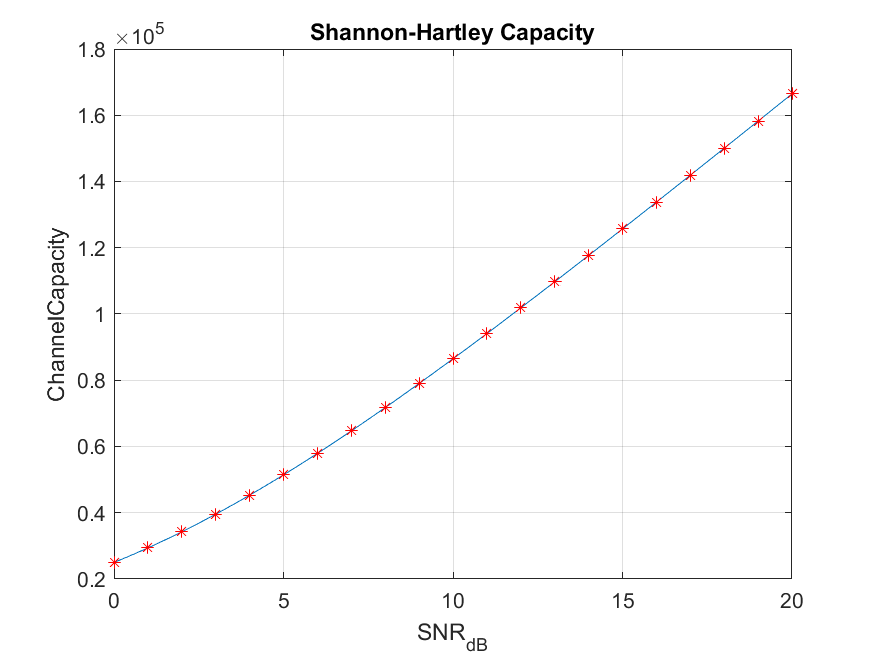
\includegraphics[width=9.5cm]{images/shannon_capacity.png}
	\caption{Shannon Capacity.}
	\label{fig:shannon}
\end{figure}

Figure \ref{fig:shannon}, show us a we had expected, while the SNR is increasing, the channel capacity increases. 
In this practice we noticed that this occurs both, when separating the transmisor and receptor, and because  of  other signals interfering like WIFI, LTE, 5G, microwaves, walls, etc. 
